 % % % % % % % % % % % % % % % % % % % % % % % % % % % % % % % % % % % %
 % % % % % % % % % % % % % % % % % % % % % % % % % % % % % % % % % % % %
 % % % % % % % % % % % % % % % % % % % % % % % % % % % % % % % % % % % %

\documentclass[paper=a4, fontsize=11pt]{scrartcl} 
\usepackage[T1]{fontenc} 
\usepackage{fourier} 
\usepackage{graphicx}
\usepackage[english]{babel} 
\usepackage{amsmath,amsfonts,amsthm} 
\usepackage{listings}
\usepackage{sectsty} 
\allsectionsfont{\centering \normalfont\scshape} 
\usepackage{fancyhdr} % Custom headers and footers

 % % % % % % % % % % % % % % % % % % % % % % % % % % % % % % % % % % % %

\pagestyle{fancyplain} 
\fancyhead{} 
\fancyfoot[L]{} 
\fancyfoot[C]{} 
\fancyfoot[R]{\thepage} 
\renewcommand{\headrulewidth}{0pt} 
\renewcommand{\footrulewidth}{0pt} 
\setlength{\headheight}{13.6pt} 
\numberwithin{equation}{section} 
\numberwithin{figure}{section} 
\numberwithin{table}{section}
\setlength\parindent{0pt} 

 % % % % % % % % % % % % % % % % % % % % % % % % % % % % % % % % % % % %

\newcommand{\horrule}[1]{\rule{\linewidth}{#1}}  
 
 % % % % % % % % % % % % % % % % % % % % % % % % % % % % % % % % % % % %

\title{	
\normalfont \normalsize 
\textsc{Barcelona Graduate School of Economics - Data Science} \\ [25pt]
\horrule{2pt} \\[0.5cm] 
\huge Deep Feature Learning for (Random) Forest Cover Type Prediction  \\ 
\horrule{2pt} \\[0.5cm] 
}

\author{J\'essica Leal, Tim Kreienkamp and Philipp Schmidt} 
\date{}



 % % % % % % % % % % % % % % % % % % % % % % % % % % % % % % % % % % % %


\begin{document}



 % % % % % % % % % % % % % % % % % % % % % % % % % % % % % % % % % % % %


\maketitle
\textbf{Abstract:} \\
From a seven-class training data with 50,000 observations we try to find the best predictive model using different Machine Learning algorithm such as K-nearest neighbors, Support Vector Machine, Random Forest and Random Forest with deep learning. Our aim is to best predict this seven-class data set with 100,000 observations. For each model, we perform a 10-fold cross validation in order to assess the performance of our classifier in the training data set. After estimating the best hyperparameters for each model - with cross-validation - and comparing the train performance, we consider the Random Forest with deep feature learning is the best type of algorithm which can predict better our data. 


 % % % % % % % % % % % % % % % % % % % % % % % % % % % % % % % % % % % %



\section{Introduction}
\subsection{Dataset Characteristics}
In this project, we work with a training data set of 50,000 observations - with labels - and a testing set - without labels - of 100,000 observations. Our aim is to predict a seven-class variable in which each label is a different type of forest cover using cartographic variables. We have 10 numeric variables presented in a raw manner that needed to be scaled, and 44 binary variables for qualitative aspects of the forest such as the wilderness of that forest and the type of soil. 

\newpage



 % % % % % % % % % % % % % % % % % % % % % % % % % % % % % % % % % % % %
\subsection{Baseline}
Before considering a unique and a priori thought best classifier, we attempted to model our data with different other classifier such as the K-NN and the SVM in order to mark us a benchmark for future steps in classification.


 % % % % % % % % % % % % % % % % % % % % % % % % % % % % % % % % % % % %

\section{Exploratory Analysis}



 % % % % % % % % % % % % % % % % % % % % % % % % % % % % % % % % % % % %


\section{Experiments}

\subsection{K-Nearest Neighbor}

With this method, we try to classify each new observation taking into consideration the majority label from its k-nearest neighbor - in our case using the Euclidean distance. In order to see which hyperparameter k we should use, we use 10-fold cross-validation with different values of k, and we see that considering the label from the training set as a factor or as an integer does not affect our results. In Figure 3.1. and 3.2 we can see that the patter of the error in cross-validation for different values of the hyperparameter k is the same, and in both cases the best k to be chosen is 3. In the case in which Y is a factor, we get an error of 22.01\%; and when Y is an integer we get an error of 22.066\%. We consider the error is quite high in the training set, so this is one of the reasons why we decided to extend our models to take into account. 
\begin{figure}
    \centering
    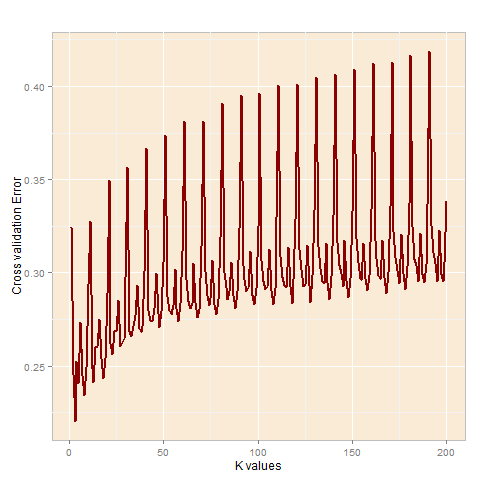
\includegraphics[width=0.8\textwidth]{ECV_factor.png}
    \caption{\textbf{Error of Cross Calidation when Y is a factor}}
    \label{fig:ECV_factor}
    \centering
    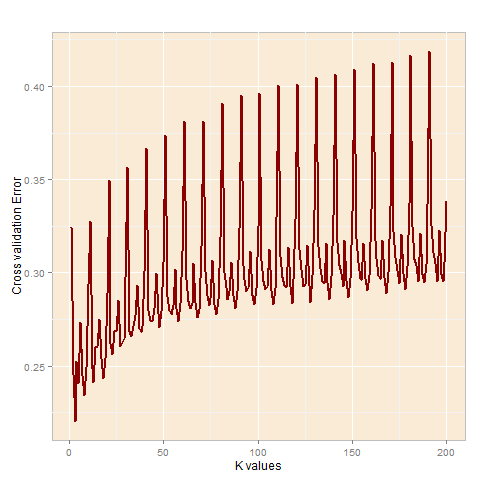
\includegraphics[width=0.8\textwidth]{ECV_factor.png}
    \caption{\textbf{Error of Cross Calidation when Y is an integer}}
    \label{fig:ECV_notfactor}
\end{figure}


 % % % % % % % % % % % % % % % % % % % % % % % % % % % % % % % % % % % %


\subsection{Support Vector Machine}
We also try to approximate to predict the labels of this data set by separating the space into halfspaces with the largest margin possible. 

\begin{figure}
    \centering
    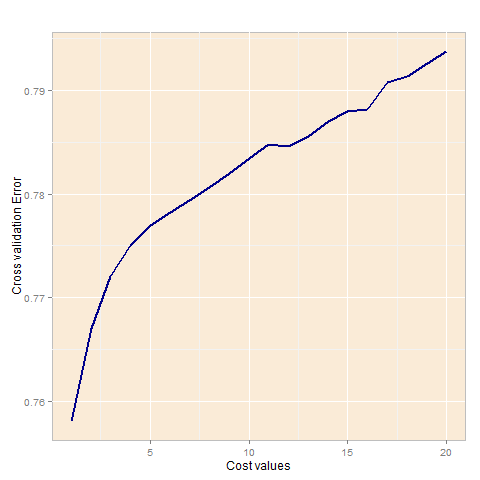
\includegraphics[width=0.8\textwidth]{SVMcost.png}
    \caption{\textbf{Accuracy of Cross Calidation for SVM}}
    \label{fig:SVM}
\end{figure}

 % % % % % % % % % % % % % % % % % % % % % % % % % % % % % % % % % % % %

\subsection{Gradient Boosting}
With this method we try to construct a classification tree of the labels why using one type of loss function: we use the multinomial distribution with a shrinkage parameter of 0.05.  

 % % % % % % % % % % % % % % % % % % % % % % % % % % % % % % % % % % % %


\subsection{Random Forest}
 We run a random forest in R with no additional parameter tuning on the full dataset. This gives us an accuracy of 0.80. From here on, we intend to make improvements.

 % % % % % % % % % % % % % % % % % % % % % % % % % % % % % % % % % % % %

\subsection{Random Forest with deep learning}

In a first set of experiments, we consider several well established classes of hypothesis functions. In particular, we consider Random Forests, Support Vector Machines, k-NN,  Gradient Tree Boosting and Neural Nets (Deep Learning). 
We first run these over a grid of hyperparameters without any feature engineering. This gives us a feeling for how well different methods are suited for the task at hand. In grid search, one evaluates a classifier over a grid, i.e. the cartesian product of several hyper parameter ranges. This process is computationally intensive, but since the data set is small, we can afford this luxury. The code for these experiments can be found in the files \lstinline{h2o_gridsearches.R}, \lstinline{svm_experiments.R} and \lstinline{knn_experiments.R}. The following figure shows the accuracy of the best model in each class. All accuracy values are obtained by a 10-fold cross validation procedure. 

We clearly see that the performance of SVM and k-NN, at least in the tried configuration with this set of features is rather disappointing. Tree based methods  and neural nets however, show - with some parameter tuning - a significant improvement over the baseline. 


 % % % % % % % % % % % % % % % % % % % % % % % % % % % % % % % % % % % %


\section{Feature Engineering and Model Tuning}
We settle on Deep Learning and Random Forests, since those performed best in the initial series of experiments. Based on our exploratory analysis, we add three new features to the data set: Horizontal Distance to Hydrology (water), Vertical Distance to Hydrology, and Total Distance to Hydrology. We feed these into the our previously best performing models, which leaves us with a slight gain in accuracy. 
Since Deep Learning seems to perform well for this data set, we try a heuristic: Why not train the Random Forest on features extracted with Deep Learning? The recent success on Deep Learning seems to be partly based on it's ability to abstract high-level concepts from the data. For this reason, Machine Learning researchers use it for feature, or representation learning. Feature learning can be done in a supervised or unsupervised manner. We use it in a supervised manner based on the heuristic: the neural net with the highest accuracy will provide the best features for our random forest. Operatively, what is done is just that the nodes of the last hidden layer in the neural net are extracted and used to transform the original feature space. The following figure shows the accuracy of all methods described: Random Forests, Deep Learning, and Random Forests with "Deep Features". 


We see that this results in a significant gain in accuracy. Apparently, Deep Learning is able to extract useful features from the data. However, in our last example we trained the random forest on 200 features. Too many features may potentially cause overfitting. This is why, in the next series of experiments, we add another layer to the neural net, where the size is significantly reduced, thus enforcing sparseness in the output. We try this with 50, 30 and 20 neurons. 


Inspecting the output shows that

 % % % % % % % % % % % % % % % % % % % % % % % % % % % % % % % % % % % %


\section{Limitations}


 % % % % % % % % % % % % % % % % % % % % % % % % % % % % % % % % % % % %

\section{Conclusions}

 % % % % % % % % % % % % % % % % % % % % % % % % % % % % % % % % % % % %


\end{document}
 % % % % % % % % % % % % % % % % % % % % % % % % % % % % % % % % % % % %
 % % % % % % % % % % % % % % % % % % % % % % % % % % % % % % % % % % % %
 % % % % % % % % % % % % % % % % % % % % % % % % % % % % % % % % % % % %